% -*- coding: utf-8 -*-
\documentclass[UTF8,a4paper,10pt]{ctexart}
\usepackage[left=3.17cm,right=3.17cm,top=2.74cm,bottom=2.74cm]{geometry}
\usepackage{amsmath}
\usepackage{amssymb}
\usepackage{graphicx}
\usepackage{float}
\usepackage{booktabs}
\usepackage{array}
\usepackage{xcolor}
\usepackage{listings}
\usepackage[colorlinks,linkcolor=black,anchorcolor=blue,urlcolor=blue]{hyperref}
\usepackage{fancyhdr}
\usepackage{tikz}
\usepackage{eso-pic}

\graphicspath{{./}{../}}
\pagestyle{fancy}
\lhead{\kaishu \leftmark}
\rhead{\kaishu 并行程序设计实验报告}
\cfoot{\thepage}
\renewcommand{\headrulewidth}{0.1pt}
\renewcommand{\footrulewidth}{0pt}
\newcommand{\HRule}{\rule{\linewidth}{0.5mm}}

\lstset{
  breaklines=true,
  basicstyle=\small\ttfamily,
  keywordstyle=\color{blue!70}\bfseries,
  commentstyle=\color{green!45!black},
  stringstyle=\color{purple!70!black},
  numbers=left,
  numberstyle=\tiny\color{gray},
  frame=single,
  columns=fullflexible
}

\newcommand{\watermark}[3]{\AddToShipoutPictureBG{
\parbox[b][\paperheight]{\paperwidth}{
\vfill
\centering
\tikz[remember picture,overlay]
  \node[rotate=#1,scale=#2] at (current page.center)
    {\textcolor{gray!20}{#3}};
\vfill}}}

\newcommand{\shot}[3]{
\begin{figure}[H]
  \centering
  \includegraphics[width=#1\textwidth]{#2}
  \caption{#3}
\end{figure}
}

\newcommand{\shotpair}[4]{
\begin{figure}[H]
  \centering
  \begin{minipage}{0.48\textwidth}
    \centering
    \includegraphics[width=\linewidth]{#1}
    \par\small #2
  \end{minipage}\hfill
  \begin{minipage}{0.48\textwidth}
    \centering
    \includegraphics[width=\linewidth]{#3}
    \par\small #4
  \end{minipage}
  \caption{AMD HIP notebook 补充截图：#2 与 #4}
\end{figure}
}

\begin{document}

\begin{titlepage}
  \begin{center}
    
\includegraphics[width=0.8\textwidth]{NKU.png}\\[1cm]
    \textsc{\Huge \kaishu{\textbf{南\ \ \ \ 开\ \ \ \ 大\ \ \ \ 学}}}\\[0.9cm]
    \textsc{\huge \kaishu{\textbf{计\ 算\ 机\ 学\ 院}}}\\[0.5cm]
    \textsc{\Large \textbf{并行程序设计实验报告}}\\[0.8cm]
    \HRule \\[0.9cm]
    {\LARGE \bfseries GPU 编程学习与矩阵 SVD 选题GPU实验}\\[0.4cm]
    \HRule \\[2.0cm]
    \textsc{\LARGE \kaishu{姓名\ :\ 邹俊轩}}\\[0.5cm]
    \textsc{\LARGE \kaishu{学号\ :\ 2412592}}\\[0.5cm]
    \textsc{\LARGE \kaishu{年级\ :\ 2024级}}\\[0.5cm]
    \textsc{\LARGE \kaishu{专业\ :\ 计算机科学与技术}}\\[0.5cm]
    \textsc{\LARGE \kaishu{指导教师\ :\ 王刚}}\\[0.5cm]
    \textsc{\Large \kaishu{代码仓库\ :\ \href{https://github.com/pointzu/gpu-svd-cuda-experiment}{github.com/pointzu/gpu-svd-cuda-experiment}}}\\[0.5cm]
    \vfill
    {\Large \today}
  \end{center}
\end{titlepage}

\newpage
\thispagestyle{empty}
\renewcommand{\abstractname}{\kaishu \large \textbf{摘要}}
\begin{abstract}
本报告围绕并行程序设计课程 GPU 编程实验与矩阵 SVD 选题展开。前半部分整理 AMD HIP 六个 notebook 中主要需要体现学习通过的代码填空、运行结果和性能分析，重点关注线程层次、访存合并、共享内存、原子操作、规约、Monte Carlo 积分和 K-Means 等 GPU 编程模式。后半部分针对 SVD 选题，说明 \texttt{bidiagonalization.cpp} 中 Householder 上二对角化阶段的 GPU 化实现思路，并结合服务器已有运行数据分析正确性、耗时分布。

\noindent\textbf{关键词：} GPU 编程；AMD HIP；SVD；Householder；CUDA/HIP；GEMV；GER；profiling
\end{abstract}

\tableofcontents
\newpage
\watermark{60}{10}{NKU}
\setcounter{page}{1}

\section{实验概述}
\subsection{实验目标}
本次实验包含两条主线。第一条主线是 AMD HIP notebook 学习实验，目标是补全 GPU 程序中的关键代码，并通过截图和性能数据说明不同并行模式的效果。第二条主线是 SVD 选题，目标是在不修改 \texttt{main.cpp/test.sh/qsub.sh} 的前提下，关注 \texttt{bidiagonalization.cpp} 中的上二对角化阶段，将其中 GEMV/GER 型 Householder 更新搬到 GPU 上，并分析加速效果和额外开销。


\section{AMD HIP Notebook 学习内容}
\subsection{Lab1：Vector Add 与线程层次}
Vector Add 的核心填空是全局线程编号计算：
\begin{lstlisting}[language=C++,title=Vector Add kernel]
int idx = blockIdx.x * blockDim.x + threadIdx.x;
if (idx < N) {
    C[idx] = A[idx] + B[idx];
}
\end{lstlisting}

对于 $N=1000$，若线程总数为 1024，则线程利用率为
\[
\frac{1000}{1024}=97.66\%.
\]
相同线程利用率不必然对应相同性能，因为实际运行还会受到 wavefront 对齐、occupancy、调度粒度和 kernel launch 固定开销影响。

\shot{0.92}{q1.png}{Lab1 GPU 检测与运行环境输出}
\shot{0.92}{q12.png}{Lab1 block size benchmark 运行结果}
\shot{0.92}{q17.png}{Lab1 sub-wavefront 对齐影响实验结果}

从截图可见，程序能够正确检测设备并完成不同 block size 的 benchmark。sub-wavefront 实验说明，过小的 block 会浪费 wavefront lane；在 AMD GPU 默认 wave32 环境下，线程块大小应尽量与 wavefront 的整数倍对齐。

\subsection{Lab2：Matrix Transpose 与访存合并}
矩阵转置中输出矩阵尺寸为 \texttt{cols x rows}，因此输出线性下标应使用输出行长度 \texttt{rows}：
\begin{lstlisting}[language=C++,title=Naive transpose write index]
output[idx * rows + idy] = input[idy * cols + idx];
\end{lstlisting}

\begin{table}[H]
\centering
\begin{tabular}{cccc}
\toprule
测试 & 维度 & 元素数 & kernel 时间 \\
\midrule
Test 1 & $16\times16$ & 256 & 0.0077 ms \\
Test 2 & $128\times32$ & 4096 & 0.0108 ms \\
Test 3 & $1\times1024$ & 1024 & 0.0087 ms \\
Test 4 & $1001\times2001$ & 2003001 & 0.2352 ms \\
\bottomrule
\end{tabular}
\caption{Matrix transpose kernel time}
\end{table}

\shot{0.92}{q21.png}{Lab2 转置测试样例运行输出}
\shot{0.92}{q25.png}{Lab2 多轮 benchmark 统计输出}
\shot{0.92}{q2c.png}{Lab2 转置访存模式分析截图}

naive transpose 能通过正确性测试，但写输出矩阵时是跨步访问，难以形成理想的 coalesced write。大规模矩阵耗时增加明显，但并不完全按元素数线性增长，说明小规模测试中固定 launch 和同步开销占比较高。

\subsection{Lab3：Histogram 与原子竞争}
Naive GPU histogram 的问题是每个 bin 对整段输入扫描一次，全局内存读次数为
\[
N\times \texttt{num\_bins}.
\]
优化版本使用 shared memory histogram：每个 block 先在共享内存中统计局部结果，再将每个 bin 的局部结果用 global atomic 合并。

\begin{table}[H]
\centering
\begin{tabular}{ccc}
\toprule
实现 & Test 2 & Test 4 \\
\midrule
Serial CPU & 2.3624 ms & 22.6050 ms \\
Naive GPU & 23.2188 ms & 2526.8180 ms \\
Optimized GPU & 0.4661 ms & 4.4517 ms \\
\bottomrule
\end{tabular}
\caption{Histogram 性能结果}
\end{table}

\shot{0.92}{q31.png}{Lab3 histogram 正确性与基础 benchmark 输出}
\shot{0.92}{q35.png}{Lab3 optimized histogram 性能对比}
\shot{0.78}{q3s.png}{Lab3 speedup 与 atomic contention 分析}

截图中的 optimized GPU 明显快于 naive GPU。优化收益来自两个方面：一是避免对全局输入数组进行 bin 数量倍的重复扫描；二是把大量竞争限制在 block 内共享内存中，减少 global atomic 压力。

\subsection{Lab4：Reduction 与 occupancy 分析}
Tree reduction 对 256 个元素进行块内规约，需要
\[
\log_2 256 = 8
\]
步。若 $N=1024$ 且 block size 为 256，则需要 $\lceil1024/256\rceil=4$ 个 block。

\begin{table}[H]
\centering
\begin{tabular}{cccc}
\toprule
Block Size & Warps/Block & Occupancy & Time \\
\midrule
64 & 2 & 100.00\% & 0.0737 ms \\
128 & 4 & 100.00\% & 0.0664 ms \\
256 & 8 & 100.00\% & 0.0641 ms \\
512 & 16 & 100.00\% & 0.0694 ms \\
1024 & 32 & 100.00\% & 0.0668 ms \\
\bottomrule
\end{tabular}
\caption{Reduction occupancy sweep}
\end{table}

\begin{table}[H]
\centering
\begin{tabular}{ccc}
\toprule
策略 & 时间 & 结果 \\
\midrule
Naive Atomic & 0.0856 ms & -74993790 \\
Tree Shared Memory & 0.0628 ms & -74993790 \\
Tree + Warp Shuffle & 0.0588 ms & -74993790 \\
Multi-Element + Tree + Shuffle & 0.0478 ms & -74993790 \\
\bottomrule
\end{tabular}
\caption{Reduction 四种策略对比}
\end{table}

\shot{0.92}{q41.png}{Lab4 reduction 基础运行输出}
\shot{0.92}{q43.png}{Lab4 occupancy sweep 结果}
\shot{0.92}{q44.png}{Lab4 多种 reduction 策略 benchmark}

所有 block size 都可以达到较高 occupancy，但最佳性能并不一定出现在最大 block size。原因是 reduction 还受到同步次数、共享内存访问、warp 内通信和最终 atomic 次数影响。multi-element + tree + shuffle 最快，说明减少全局 atomic 并利用 warp shuffle 可以进一步降低开销。

\subsection{Lab5：Monte Carlo Integration}
Atomic 版本中，每个线程把自己的样本贡献直接加到同一个全局结果：
\begin{lstlisting}[language=C++,title=Monte Carlo atomic accumulation]
double tmp = (b - a) * y_samples[idx] / n_samples;
atomicAdd(result, tmp);
\end{lstlisting}
该写法总工作量为 $O(n)$，但所有线程竞争同一个全局地址，global atomic accumulation 成为瓶颈。

Test 1 的手算结果为
\[
\sum y_i = 23.7507,\qquad
\text{result}=\frac{2}{8}\times 23.7507=5.937675.
\]

\begin{table}[H]
\centering
\begin{tabular}{ccc}
\toprule
测试 & 样本数 & 时间 \\
\midrule
Test 4 & 100000 & real 0m0.074s \\
Test 7 & 10000000 & real 0m0.878s \\
Test 8 & 100000000 & real 0m8.425s \\
\bottomrule
\end{tabular}
\caption{Monte Carlo scaling}
\end{table}

\shot{0.92}{q51.png}{Lab5 Monte Carlo 小规模样例输出}
\shot{0.92}{q54.png}{Lab5 Monte Carlo scaling 运行结果}
\shot{0.92}{q56.png}{Lab5 Performance Scaling 分析截图}

从 Test 4 到 Test 7，样本数增加 100 倍，运行时间增加约 $0.878/0.074=11.86$ 倍，并非严格线性。小规模输入中内存分配、数据拷贝和 kernel launch 固定开销占比较高；大规模输入则逐渐受内存带宽与 atomic contention 限制。

\subsection{Lab6：K-Means}
Assignment kernel 中每个点需要和所有 centroid 计算距离，因此每个线程复杂度为 $O(k)$。当 $k=100$ 时，每个点都要进行 100 次距离比较。Update kernel 使用 shared memory atomics 先在 block 内聚合，再写回 global memory，以减少 global atomic 竞争。

\[
dx^2 + dy^2 < 10^{-8}
\]
是收敛判断条件。Double buffering 将旧 centroid 和新 centroid 分开存储，既能安全比较收敛，也避免覆盖当前迭代仍需使用的数据。

\shot{0.92}{q61.png}{Lab6 K-Means 数据生成与编译}
\shot{0.92}{q63.png}{Lab6 K-Means 测试样例运行结果}
\shot{0.92}{q65.png}{Lab6 K-Means 性能分析结果}

截图显示程序能够完成数据生成、编译和测试。K-Means 的主导开销来自 assignment step，因为每个点都需要遍历全部 centroid；当输入规模、聚类中心数或迭代次数增加时，运行时间会相应增长。

\section{SVD GPU实验}
\subsection{计算流程}
SVD 框架主流程如下：
\begin{enumerate}
  \item \texttt{main.cpp} 构造测试矩阵 $A$；
  \item \texttt{to\_bidiagonal} 将 $A$ 化为上二对角矩阵 $B$，并累计正交矩阵 $U,V$；
  \item \texttt{gkh\_svd\_from\_bidiagonal} 对 $B$ 做 Golub-Kahan 迭代，使其收敛为非负降序对角矩阵；
  \item 主程序验证重构误差、正交误差、对角结构和奇异值排序。
\end{enumerate}
框架保持 $A=UBV^T$ 不变，最终 $B$ 的对角线元素即为奇异值。

\subsection{Householder 阶段的 GPU 化}
\texttt{bidiagonalization.cpp} 中的 Householder 更新可写成 GEMV 与 GER：
\[
w=v^T B_{\text{sub}},\qquad
B_{\text{sub}}\leftarrow B_{\text{sub}}-\beta v w^T.
\]
指导书要求关注外层循环 \texttt{for (int k = 0; k < n; ++k)} 中交替执行的左乘和右乘 Householder。每一步对 $B,U,V$ 分别包含 GEMV 和 GER，因此矩阵元素级更新天然适合 GPU 并行。

本实现选择手写 CUDA/HIP kernel 路线，而不是直接调用 cuBLAS。原因是框架中的 \texttt{Matrix} 类采用行主序存储，而 cuBLAS 默认列主序，直接替换容易出现转置关系错误。手写 kernel 可以保持原有行主序布局，并显式控制访存方式。

\begin{lstlisting}[language=C++,title=GPU Householder kernels]
householder_dot_cols_kernel(...)
householder_dot_rows_kernel(...)
householder_left_update_kernel(...)
householder_rows_update_kernel(...)
\end{lstlisting}

其中 \texttt{dot\_cols} 与 \texttt{dot\_rows} 对应 GEMV，分别计算 $v^T B_{\text{sub}}$ 和 $B_{\text{sub}}v$；\texttt{left\_update} 与 \texttt{rows\_update} 对应 GER，每个线程负责更新矩阵中的一个元素。代码中还保留 \texttt{SVD\_USE\_CUDA}、\texttt{SVD\_USE\_HIP} 和默认 CPU/SIMD 回退路径。

\subsection{GKH 阶段说明}
本报告只把 \texttt{to\_bidiagonal} 内部实现作为 GPU 化对象。服务器运行结果显示，GKH 迭代耗时显著大于上二对角化耗时，所以完整 SVD 的总时间仍会受到后续 CPU 侧迭代限制。

\begin{lstlisting}[language=C++,basicstyle=\scriptsize\ttfamily,title=bidiagonalization.cpp 中 SVD GPU kernel 完整代码块]
#if defined(SVD_USE_HIP) && defined(__HIPCC__)
#include <hip/hip_runtime.h>
#define SVD_CUDA_ENABLED 1
#define cudaError_t hipError_t
#define cudaSuccess hipSuccess
#define cudaMalloc hipMalloc
#define cudaFree hipFree
#define cudaMemcpy hipMemcpy
#define cudaMemcpyHostToDevice hipMemcpyHostToDevice
#define cudaMemcpyDeviceToHost hipMemcpyDeviceToHost
#define cudaGetDeviceCount hipGetDeviceCount
#define cudaGetLastError hipGetLastError
#define cudaDeviceSynchronize hipDeviceSynchronize
#elif defined(SVD_USE_CUDA) && defined(__CUDACC__)
#include <cuda_runtime.h>
#define SVD_CUDA_ENABLED 1
#else
#define SVD_CUDA_ENABLED 0
#endif

#if SVD_CUDA_ENABLED
__global__ void householder_dot_cols_kernel(const double *matrix, const double *v,
                                            double *out, int rows, int cols,
                                            int row0, int col0,
                                            int sub_rows, int sub_cols)
{
    extern __shared__ double partial[];
    const int col = blockIdx.x;
    const int tid = threadIdx.x;

    double sum = 0.0;
    if (col < sub_cols)
    {
        for (int i = tid; i < sub_rows; i += blockDim.x)
            sum += v[i] * matrix[(row0 + i) * cols + (col0 + col)];
    }
    partial[tid] = sum;
    __syncthreads();

    for (int stride = blockDim.x / 2; stride > 0; stride >>= 1)
    {
        if (tid < stride)
            partial[tid] += partial[tid + stride];
        __syncthreads();
    }

    if (tid == 0 && col < sub_cols)
        out[col] = partial[0];
}

__global__ void householder_dot_rows_kernel(const double *matrix, const double *v,
                                            double *out, int rows, int cols,
                                            int row0, int col0,
                                            int sub_rows, int sub_cols)
{
    extern __shared__ double partial[];
    const int row = blockIdx.x;
    const int tid = threadIdx.x;

    double sum = 0.0;
    if (row < sub_rows)
    {
        for (int j = tid; j < sub_cols; j += blockDim.x)
            sum += matrix[(row0 + row) * cols + (col0 + j)] * v[j];
    }
    partial[tid] = sum;
    __syncthreads();

    for (int stride = blockDim.x / 2; stride > 0; stride >>= 1)
    {
        if (tid < stride)
            partial[tid] += partial[tid + stride];
        __syncthreads();
    }

    if (tid == 0 && row < sub_rows)
        out[row] = partial[0];
}

__global__ void householder_left_update_kernel(double *matrix, const double *v,
                                               const double *w, double beta,
                                               int rows, int cols, int row0,
                                               int col0, int sub_rows,
                                               int sub_cols)
{
    const int col = blockIdx.x * blockDim.x + threadIdx.x;
    const int row = blockIdx.y * blockDim.y + threadIdx.y;
    if (row < sub_rows && col < sub_cols)
        matrix[(row0 + row) * cols + (col0 + col)] -= beta * v[row] * w[col];
}

__global__ void householder_rows_update_kernel(double *matrix, const double *v,
                                               const double *w, double beta,
                                               int rows, int cols, int row0,
                                               int col0, int sub_rows,
                                               int sub_cols)
{
    const int col = blockIdx.x * blockDim.x + threadIdx.x;
    const int row = blockIdx.y * blockDim.y + threadIdx.y;
    if (row < sub_rows && col < sub_cols)
        matrix[(row0 + row) * cols + (col0 + col)] -= beta * w[row] * v[col];
}

static bool gpu_householder_left(Matrix &B, Matrix &U, int k,
                                 const std::vector<double> &v, double beta)
{
    if (!cuda_device_ready())
        return false;

    const int m = B.rows();
    const int n = B.cols();
    const int sub_rows = m - k;
    const int sub_cols = n - k;
    const int threads = 256;
    const dim3 tile(16, 16);
    const dim3 b_grid((sub_cols + tile.x - 1) / tile.x,
                      (sub_rows + tile.y - 1) / tile.y);
    const dim3 u_grid((sub_rows + tile.x - 1) / tile.x,
                      (m + tile.y - 1) / tile.y);

    DeviceBuffer d_B(B.size()), d_U(U.size()), d_v(v.size());
    DeviceBuffer d_wB(sub_cols), d_wU(m);
    if (!d_B.ok() || !d_U.ok() || !d_v.ok() || !d_wB.ok() || !d_wU.ok())
        return false;

    if (!copy_to_device(d_B, B.data()) || !copy_to_device(d_U, U.data()) ||
        !copy_to_device(d_v, v.data()))
        return false;

    householder_dot_cols_kernel<<<sub_cols, threads, threads * sizeof(double)>>>(
        d_B.get(), d_v.get(), d_wB.get(), m, n, k, k, sub_rows, sub_cols);
    if (!cuda_ok(cudaGetLastError()))
        return false;

    householder_left_update_kernel<<<b_grid, tile>>>(
        d_B.get(), d_v.get(), d_wB.get(), beta, m, n, k, k, sub_rows, sub_cols);
    if (!cuda_ok(cudaGetLastError()))
        return false;

    householder_dot_rows_kernel<<<m, threads, threads * sizeof(double)>>>(
        d_U.get(), d_v.get(), d_wU.get(), m, m, 0, k, m, sub_rows);
    if (!cuda_ok(cudaGetLastError()))
        return false;

    householder_rows_update_kernel<<<u_grid, tile>>>(
        d_U.get(), d_v.get(), d_wU.get(), beta, m, m, 0, k, m, sub_rows);
    if (!cuda_ok(cudaGetLastError()) || !cuda_ok(cudaDeviceSynchronize()))
        return false;

    std::vector<double> host_B(B.size()), host_U(U.size());
    if (!copy_to_host(host_B.data(), d_B) || !copy_to_host(host_U.data(), d_U))
        return false;
    std::copy(host_B.begin(), host_B.end(), B.data());
    std::copy(host_U.begin(), host_U.end(), U.data());
    return true;
}

static bool gpu_householder_right(Matrix &B, Matrix &V, int k,
                                  const std::vector<double> &v, double beta)
{
    if (!cuda_device_ready())
        return false;

    const int m = B.rows();
    const int n = B.cols();
    const int sub_rows = m - k;
    const int sub_cols = n - k - 1;
    const int threads = 256;
    const dim3 tile(16, 16);
    const dim3 b_grid((sub_cols + tile.x - 1) / tile.x,
                      (sub_rows + tile.y - 1) / tile.y);
    const dim3 v_grid((sub_cols + tile.x - 1) / tile.x,
                      (n + tile.y - 1) / tile.y);

    DeviceBuffer d_B(B.size()), d_V(V.size()), d_vec(v.size());
    DeviceBuffer d_wB(sub_rows), d_wV(n);
    if (!d_B.ok() || !d_V.ok() || !d_vec.ok() || !d_wB.ok() || !d_wV.ok())
        return false;

    if (!copy_to_device(d_B, B.data()) || !copy_to_device(d_V, V.data()) ||
        !copy_to_device(d_vec, v.data()))
        return false;

    householder_dot_rows_kernel<<<sub_rows, threads, threads * sizeof(double)>>>(
        d_B.get(), d_vec.get(), d_wB.get(), m, n, k, k + 1, sub_rows, sub_cols);
    if (!cuda_ok(cudaGetLastError()))
        return false;

    householder_rows_update_kernel<<<b_grid, tile>>>(
        d_B.get(), d_vec.get(), d_wB.get(), beta, m, n, k, k + 1, sub_rows, sub_cols);
    if (!cuda_ok(cudaGetLastError()))
        return false;

    householder_dot_rows_kernel<<<n, threads, threads * sizeof(double)>>>(
        d_V.get(), d_vec.get(), d_wV.get(), n, n, 0, k + 1, n, sub_cols);
    if (!cuda_ok(cudaGetLastError()))
        return false;

    householder_rows_update_kernel<<<v_grid, tile>>>(
        d_V.get(), d_vec.get(), d_wV.get(), beta, n, n, 0, k + 1, n, sub_cols);
    if (!cuda_ok(cudaGetLastError()) || !cuda_ok(cudaDeviceSynchronize()))
        return false;

    std::vector<double> host_B(B.size()), host_V(V.size());
    if (!copy_to_host(host_B.data(), d_B) || !copy_to_host(host_V.data(), d_V))
        return false;
    std::copy(host_B.begin(), host_B.end(), B.data());
    std::copy(host_V.begin(), host_V.end(), V.data());
    return true;
}
#endif
\end{lstlisting}

\section{服务器运行与结果分析}
\subsection{服务器与本地运行结果}
服务器侧在 \texttt{master\_ubss2} 上使用种子 $2412592$ 完成了 O2 优化运行，输出文件为 \texttt{test\_O2\_4cores.o}：
\begin{lstlisting}[language=bash,title=Server O2 run]
bash test.sh 5 1 4 -O O2 -s 2412592
\end{lstlisting}

\begin{table}[H]
\centering
\begin{tabular}{lcc}
\toprule
指标 & 服务器 O2 结果 & 说明 \\
\midrule
通过样例数 & 5 / 5 & 全部 PASS \\
$1000\times1000$ 上二对角化耗时 & 3456.54 ms & Householder 阶段 \\
$1000\times1000$ GKH 耗时 & 23967.5 ms & 后续迭代阶段 \\
总上二对角化耗时 & 3456.61 ms & 5 个测试合计 \\
总 GKH 耗时 & 23968.4 ms & 5 个测试合计 \\
\bottomrule
\end{tabular}
\caption{服务器 O2 运行结果}
\end{table}

本地 Windows 环境也使用同一份 \texttt{GPU/code} 代码重新编译并运行 CPU baseline：
\begin{lstlisting}[language=bash,title=Local CPU run]
g++ -std=c++17 -O2 -pthread main.cpp bidiagonalization.cpp gkh.cpp -o main_local.exe
./main_local.exe 2412592
\end{lstlisting}
本地运行同样得到 5 / 5 PASS，其中 $1000\times1000$ 样例上二对角化耗时约为 2824.13 ms，GKH 迭代耗时约为 5234.98 ms；5 个测试合计上二对角化耗时为 2824.13 ms，GKH 迭代耗时为 5238.27 ms。本地 \texttt{nvidia-smi} 显卡为 NVIDIA GeForce RTX 4060 Laptop GPU，驱动版本为 610.47，CUDA UMD 版本为 13.3。

\subsection{本地 NVIDIA GPU 测试}
补充使用当前 Python 环境中的 \texttt{torch 2.11.0+cu128} 运行 CUDA smoke test。测试脚本为 \texttt{GPU/code/local\_nvidia\_gpu\_smoke.py}，输出保存为 \texttt{local\_nvidia\_gpu\_smoke.json}：
\begin{lstlisting}[language=bash,title=Local NVIDIA GPU  test]
python local_nvidia_gpu_smoke.py
\end{lstlisting}

\begin{table}[H]
\centering
\begin{tabular}{lcc}
\toprule
项目 & 结果 & 说明 \\
\midrule
GPU & NVIDIA GeForce RTX 4060 Laptop GPU & 8 GB 级显存 \\
Compute Capability & 8.9 & Ada Lovelace 移动端 GPU \\
PyTorch CUDA & 12.8 & \texttt{torch 2.11.0+cu128} \\
$4096\times4096$ CPU matmul & 285.372 ms & CPU 对照 \\
$4096\times4096$ GPU matmul & 23.599 ms & CUDA Event 计时 \\
矩阵乘加速比 & 12.09$\times$ & CPU / GPU \\
Householder-like 更新 & 2.523 ms & GEMV + GER 型微基准 \\
\bottomrule
\end{tabular}
\caption{本地 NVIDIA GPU  test 结果}
\end{table}

该测试证明本地 RTX 4060 可以通过 CUDA 路径正常执行大规模矩阵运算，并且对 GEMV/GER 风格的 Householder-like 更新也能给出毫秒级执行时间。

\subsection{本地 nvcc CUDA C++ SVD 运行}
在完成 CUDA Toolkit 13.3 与 Visual Studio 2022 Build Tools 安装后，本地已能使用 \texttt{nvcc} 编译 \texttt{bidiagonalization.cpp} 中真正嵌入 SVD 程序的 CUDA kernel。由于 \texttt{main.cpp} 与 \texttt{gkh.cpp} 是普通 C++ 代码，而 \texttt{bidiagonalization.cpp} 内含 \texttt{\_\_global\_\_} kernel，本次采用分步编译：普通 C++ 文件由 MSVC 编译，GPU kernel 文件由 \texttt{nvcc -x cu} 编译，最后再链接为 \texttt{svd\_cuda.exe}。

\begin{lstlisting}[language=bash,title=Local nvcc CUDA C++ build]
cl /std:c++17 /O2 /EHsc /DNOMINMAX /utf-8 /c main.cpp gkh.cpp
nvcc -x cu -std=c++17 -O2 -DSVD_USE_CUDA -DSVD_PROFILE_GPU ^
  -Xcompiler "/utf-8 /EHsc /DNOMINMAX" ^
  -c bidiagonalization.cpp -o bidiagonalization_cuda.obj
nvcc main.obj gkh.obj bidiagonalization_cuda.obj -o svd_cuda.exe
svd_cuda.exe 2412592 > local_nvcc_cuda_run.txt 2>&1
\end{lstlisting}

\begin{table}[H]
\centering
\begin{tabular}{lc}
\toprule
项目 & 本地 CUDA C++ 结果 \\
\midrule
GPU & NVIDIA GeForce RTX 4060 Laptop GPU \\
显存 & 8188 MiB \\
驱动版本 & 610.47 \\
CUDA Toolkit & 13.3, \texttt{nvcc} 13.3.33 \\
MSVC Build Tools & Visual Studio 2022 BuildTools 17.14.35 \\
随机种子 & 2412592 \\
通过样例数 & 5 / 5 \\
\bottomrule
\end{tabular}
\caption{本地 nvcc 编译链与 CUDA C++ 运行环境}
\end{table}

\begin{table}[H]
\centering
\begin{tabular}{lcc}
\toprule
指标 & 本地 CPU O2 & 本地 CUDA C++ \\
\midrule
$1000\times1000$ 上二对角化耗时 & 2824.13 ms & 17315.3 ms \\
$1000\times1000$ GKH 耗时 & 5234.98 ms & 5983.64 ms \\
总上二对角化耗时 & 2824.13 ms & 17730.1 ms \\
总 GKH 耗时 & 5238.27 ms & 5987.52 ms \\
通过样例数 & 5 / 5 & 5 / 5 \\
\bottomrule
\end{tabular}
\caption{本地 CPU O2 与 nvcc CUDA C++ 端到端结果对比}
\end{table}

\begin{figure}[H]
  \centering
  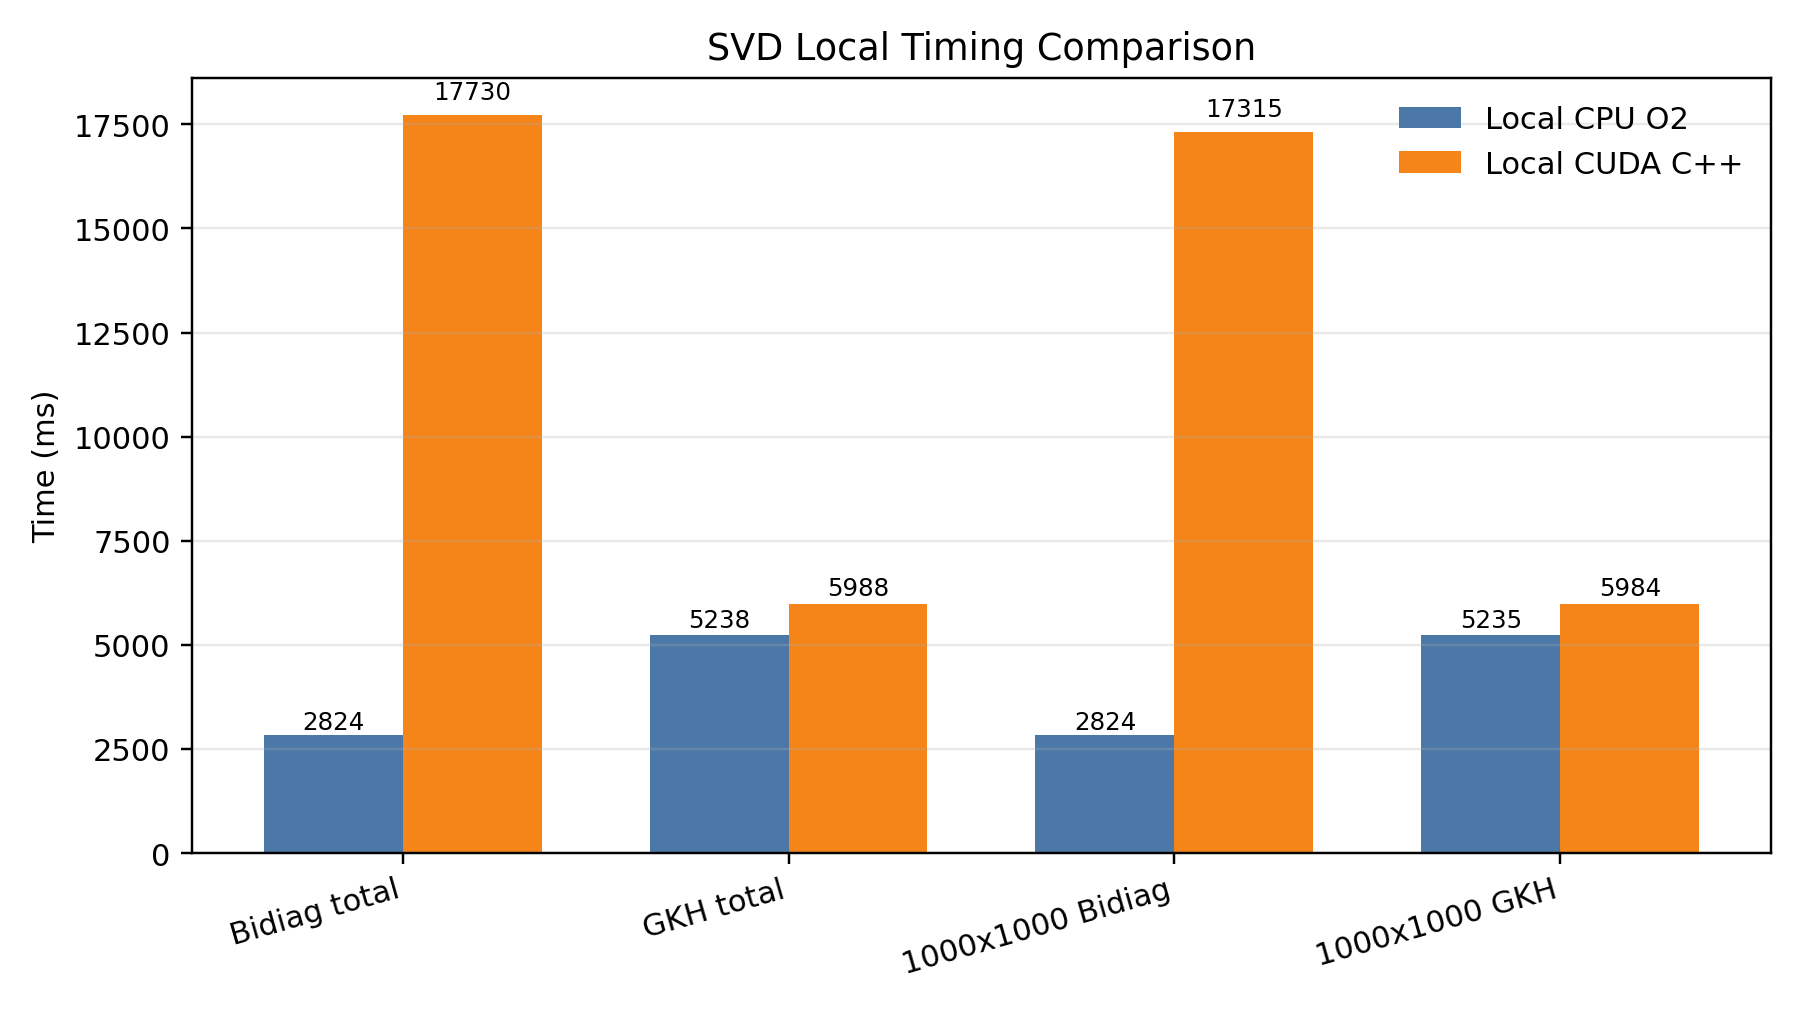
\includegraphics[width=0.92\textwidth]{svd_timing_compare.png}
  \caption{本地 CPU O2 与 CUDA C++ SVD 耗时对比图}
\end{figure}

\begin{table}[H]
\centering
\begin{tabular}{lcc}
\toprule
GPU profile 指标 & 数值 & 说明 \\
\midrule
H2D 拷贝时间 & 3825.486 ms & Host 到 Device \\
D2H 拷贝时间 & 3097.562 ms & Device 到 Host \\
kernel 同步时间 & 431.515 ms & GPU kernel 执行与同步 \\
H2D 数据量 & 30479.484 MB & 累计传输量 \\
D2H 数据量 & 30471.852 MB & 累计传输量 \\
左 Householder 调用 & 1026 次 & \texttt{gpu\_householder\_left} \\
右 Householder 调用 & 1019 次 & \texttt{gpu\_householder\_right} \\
\bottomrule
\end{tabular}
\caption{\texttt{SVD\_GPU\_PROFILE} 输出的本地 CUDA 运行统计}
\end{table}

\begin{figure}[H]
  \centering
  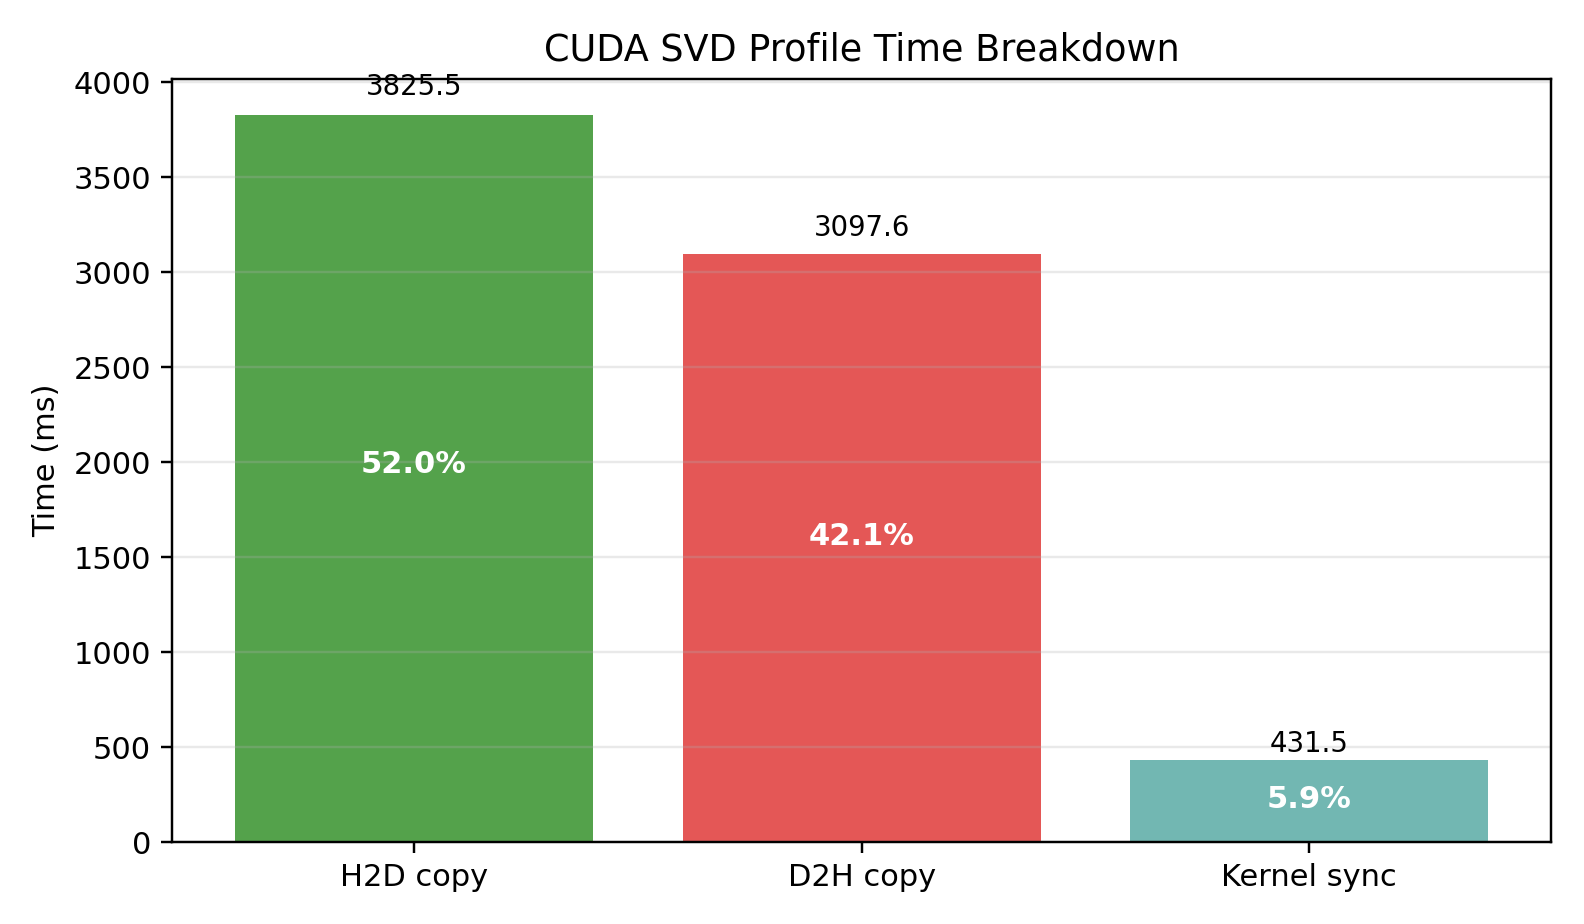
\includegraphics[width=0.82\textwidth]{svd_cuda_profile_time.png}
  \caption{本地 CUDA SVD profile 时间分解图}
\end{figure}

从 profile 可见，kernel 本身累计同步时间为 431.515 ms，低于本地 CPU O2 的上二对角化总时间；但当前实现为了兼容原有 \texttt{Matrix} 接口，每次左/右 Householder 都重新分配设备缓冲并进行整矩阵 H2D/D2H 拷贝，累计传输量超过 60 GB。最终 CUDA C++ 端到端上二对角化耗时反而达到 17730.1 ms，约为本地 CPU O2 的 $17730.1/2824.13\approx6.28$ 倍。这说明手写 GPU kernel 的计算部分已经能够工作，但数据驻留和传输策略是当前版本的主要瓶颈。

\subsection{VTune 与 AMD uProf profiling}
使用 VTune 对 \texttt{main\_local.exe} 进行 hotspots 采样：

\begin{table}[H]
\centering
\begin{tabular}{lcc}
\toprule
热点函数 & CPU Time & 占比 \\
\midrule
\texttt{apply\_right\_cols\_range} & 3.539 s & 37.4\% \\
\texttt{main\_local.exe} 未细分符号 & 1.626 s & 17.2\% \\
\texttt{simd\_add\_scaled} & 1.610 s & 17.0\% \\
\texttt{simd\_dot} & 1.004 s & 10.6\% \\
\texttt{cleanup\_bidiagonal} & 0.921 s & 9.7\% \\
其他 & 0.755 s & 8.0\% \\
\bottomrule
\end{tabular}
\caption{本地 VTune hotspots 采样结果}
\end{table}

\begin{figure}[H]
  \centering
  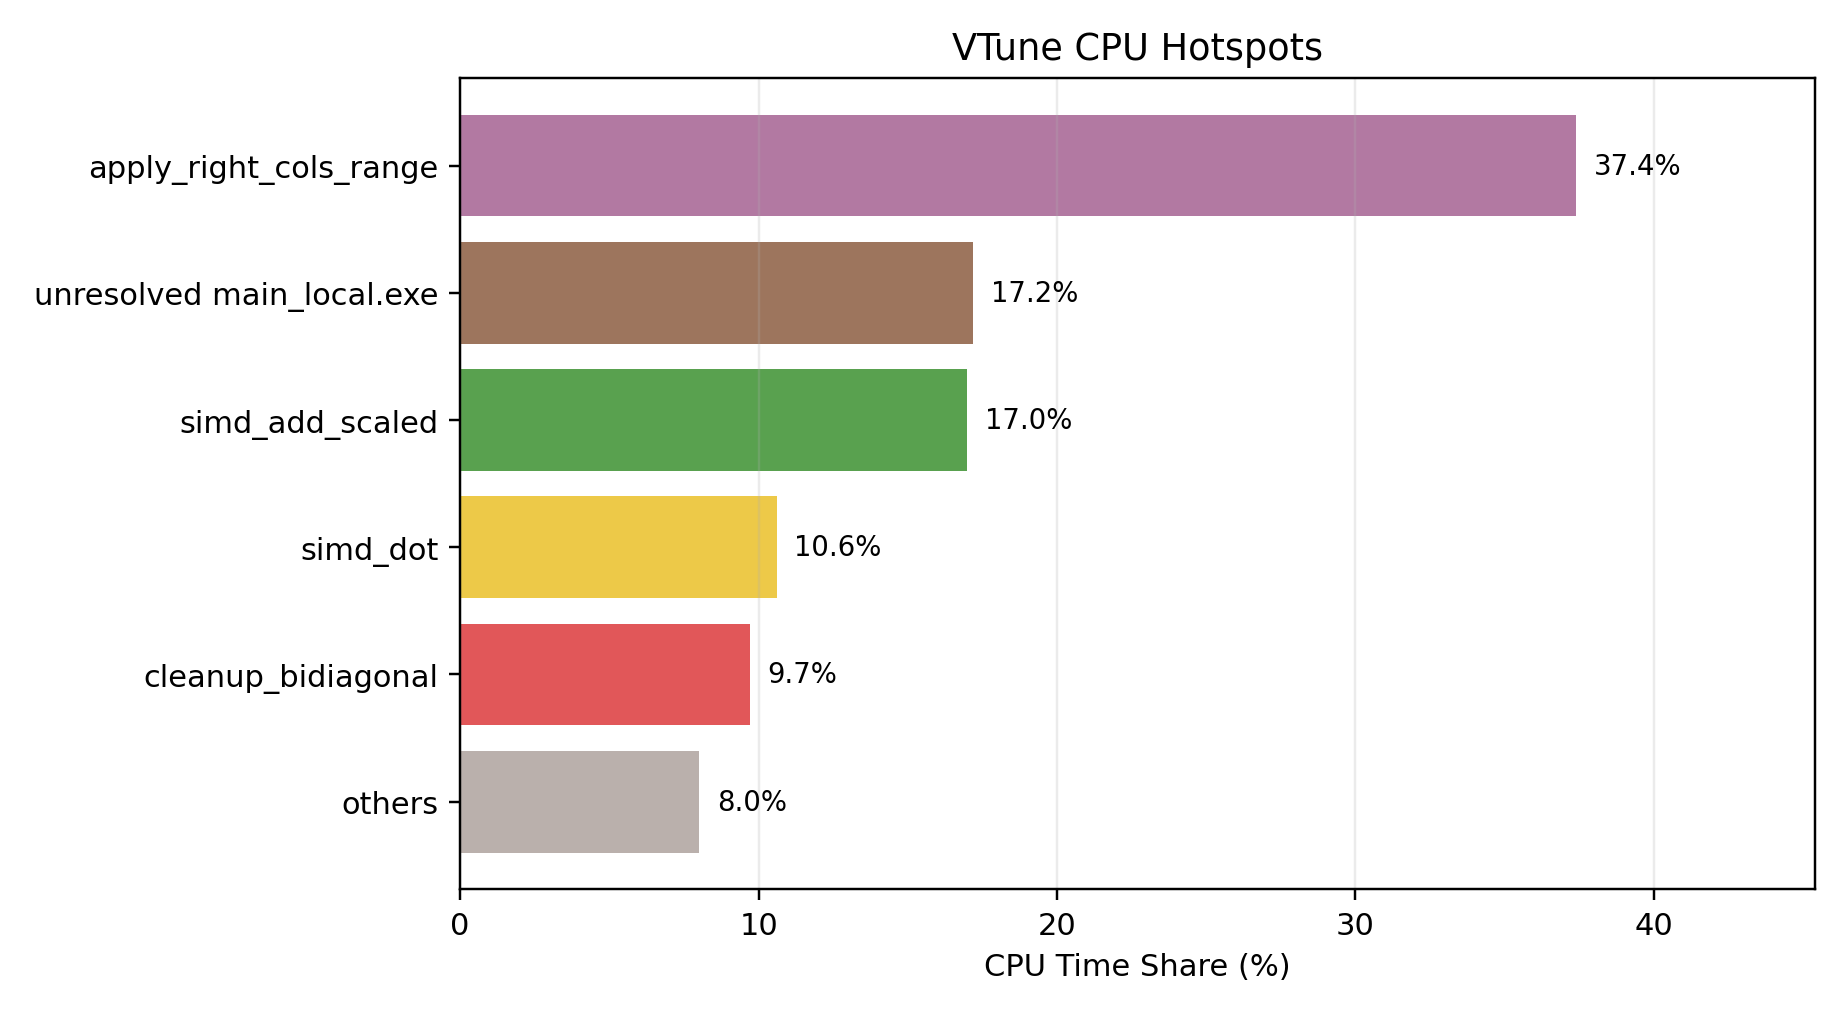
\includegraphics[width=0.92\textwidth]{svd_vtune_hotspots.png}
  \caption{VTune CPU hotspots 占比图}
\end{figure}

VTune 报告显示总 elapsed time 为 10.019 s，CPU time 为 9.455 s，采样方式为 user-mode sampling and tracing。热点主要集中在 \texttt{bidiagonalization.cpp} 的 CPU Householder 路径，尤其是右侧列更新、SIMD 向量加法、SIMD 点积和双对角清理。这说明 CPU baseline 的性能瓶颈落在上二对角化内部的 GEMV/GER 型更新循环中，也正对应本实验选择 GPU 化的核心动机。


\subsection{结果分析}
服务器 O2 结果中，$1000\times1000$ 样例的 GKH 耗时约为上二对角化耗时的
\[
\frac{23967.5}{3456.54}\approx6.93
\]
倍；本地 CPU 对照运行中，该比例约为
\[
\frac{5234.98}{2824.13}\approx1.85
\]
倍。两组数据的绝对时间受硬件、编译器和运行环境影响较大，但共同说明完整 SVD 并不只由上二对角化决定，后续 GKH 迭代仍会限制总加速。因此即使 \texttt{to\_bidiagonal} 内部 GEMV/GER 已经接入 GPU 路径，完整程序的端到端加速也可能被 CPU 侧 GKH 阶段抵消。

此外，本地 nvcc 运行进一步验证了这一点：\texttt{SVD\_GPU\_PROFILE} 中 kernel 同步时间只有 431.515 ms，但 H2D/D2H 拷贝时间合计约为 6923.048 ms，且每次 Householder 都伴随设备内存分配、整矩阵复制和同步。若矩阵不能长期驻留在 GPU 显存中，通信与调度开销会抵消 kernel 并行带来的收益。说明后续优化方向应优先考虑持久化设备端矩阵、批量执行多个 Householder 更新以及减少全矩阵回拷。

\section{总结}
本报告整理了 AMD HIP 六个 notebook 的关键代码填空、截图结果和性能分析，并针对 SVD 选题说明了 Householder 上二对角化阶段的 GPU 化实现。代码层面，\texttt{bidiagonalization.cpp} 已经提供手写 CUDA/HIP kernel 路径，覆盖 GEMV/GER 型更新。服务器 O2 运行在学号种子 $2412592$ 下通过全部 5 个测试样例，说明当前实现保持了 SVD 分解正确性。本地进一步完成 CUDA Toolkit 13.3 与 Visual Studio 2022 Build Tools 编译链配置，使用 \texttt{nvcc} 成功构建并运行 \texttt{svd\_cuda.exe}，CUDA C++ 路径同样 5 / 5 PASS。profiling 显示 kernel 累计同步时间为 431.515 ms，但 H2D/D2H 拷贝时间合计约 6923.048 ms，导致端到端上二对角化慢于本地 CPU O2。该结果说明 GPU kernel 的计算正确性已经得到验证，而性能瓶颈主要来自当前实现的数据搬运和设备内存生命周期管理。

\section{SVD 选题 AI 问答记录}

\shot{0.92}{../../ai1.png}{SVD AI 问答截图 1}
\shot{0.92}{../../ai2.png}{SVD AI 问答截图 2}
\shot{0.92}{../../ai3.png}{SVD AI 问答截图 3}

\section{截图与材料清单}
\begin{table}[H]
\centering
\begin{tabular}{p{0.18\textwidth}p{0.33\textwidth}p{0.39\textwidth}}
\toprule
编号 & 已插入截图 & 内容 \\
\midrule
1 & \texttt{q1,q12,q17} & Lab1 设备检测、block size、sub-wavefront \\
2 & \texttt{q21,q25,q2c} & Lab2 转置 benchmark 与访存分析 \\
3 & \texttt{q31,q35,q3s} & Lab3 histogram benchmark 与 speedup \\
4 & \texttt{q41,q43,q44} & Lab4 reduction 与 occupancy sweep \\
5 & \texttt{q51,q54,q56} & Lab5 Monte Carlo scaling \\
6 & \texttt{q61,q63,q65} & Lab6 K-Means 编译、测试与性能 \\
7 & \texttt{test\_O2\_4cores.o}、\texttt{local\_cpu\_O2.txt}、\texttt{local\_nvidia\_gpu\_smoke.json}、\texttt{local\_nvcc\_cuda\_run.txt}、\texttt{local\_nvcc\_build.log}、\texttt{vtune\_summary.txt} & 服务器 O2 结果、本地 CPU 对照、本地 NVIDIA GPU smoke test、本地 nvcc CUDA C++ 运行与 profile、本地 VTune hotspots \\
8 & \texttt{svd\_timing\_compare.png}、\texttt{svd\_cuda\_profile\_time.png}、\texttt{svd\_vtune\_hotspots.png} & 数据分析图表：端到端耗时对比、CUDA profile 分解、CPU hotspots 占比 \\
9 & \texttt{ai1.png, ai2.png, ai3.png} & SVD AI 问答过程截图 \\
\bottomrule
\end{tabular}
\caption{截图与材料清单}
\end{table}

\section{AMD Notebook 补充截图附录}
\shotpair{1.png}{1.png}{12.png}{12.png}
\shotpair{13.png}{13.png}{14.png}{14.png}
\shotpair{15.png}{15.png}{16.png}{16.png}
\shotpair{l2.png}{l2.png}{l22.png}{l22.png}
\shotpair{l23.png}{l23.png}{l31.png}{l31.png}
\shotpair{l32.png}{l32.png}{l33.png}{l33.png}
\shotpair{l34.png}{l34.png}{l35.png}{l35.png}
\shotpair{l41.png}{l41.png}{l43.png}{l43.png}
\shotpair{l44.png}{l44.png}{l45.png}{l45.png}
\shotpair{l46.png}{l46.png}{l47.png}{l47.png}
\shotpair{l51.png}{l51.png}{l54.png}{l54.png}
\shotpair{l55.png}{l55.png}{l61.png}{l61.png}
\shotpair{l62.png}{l62.png}{l63.png}{l63.png}
\shotpair{l64.png}{l64.png}{l66.png}{l66.png}
\shotpair{lq2.png}{lq2.png}{p25.png}{p25.png}
\shotpair{q15.png}{q15.png}{q16.png}{q16.png}
\shotpair{q1c.png}{q1c.png}{q22QQ20260619-224052.png}{q22QQ20260619-224052.png}
\shotpair{q23.png}{q23.png}{q24.png}{q24.png}
\shotpair{q32.png}{q32.png}{q33.png}{q33.png}
\shotpair{q34.png}{q34.png}{q3c.png}{q3c.png}
\shotpair{q42.png}{q42.png}{q52.png}{q52.png}
\shotpair{q53.png}{q53.png}{q55.png}{q55.png}
\shotpair{q62.png}{q62.png}{q64.png}{q64.png}

\begin{thebibliography}{9}
\bibitem{gpu-lab}
并行程序设计课程组. 2026 并行程序设计 Lab5 GPU 编程.
\bibitem{svd}
Golub, G. H. and Van Loan, C. F. Matrix Computations.
\end{thebibliography}
\end{document}
